%----------------------------------------------------------------------------------------
%	PRESENTATION SLIDES
%----------------------------------------------------------------------------------------

%------------------------------------------------
\section{Introduction to Kitaev quantum spin liquid.} % Sections can be created in order to organize your presentation into discrete blocks, all sections and subsections are automatically printed in the table of contents as an overview of the talk
%------------------------------------------------

\begin{frame}
\centerline{1. Introduction to Kitaev quantum spin liquid.}
\end{frame}


% \begin{frame}{Fractionalized excitations in spin-1/2 Heisenberg AFM chain}
% \begin{figure}
% \centering
%     \begin{minipage}[c]{.45\textwidth}
%         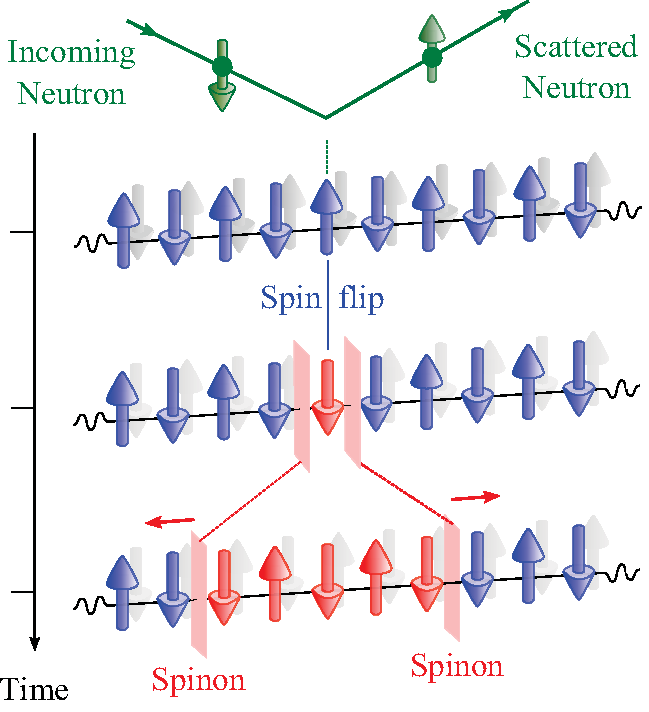
\includegraphics[width = 1\textwidth]{figures/caux-nature-physics-cartoon.png}  
%     \end{minipage}
% \end{figure}
% A single spin flip generates two unhappy bonds. The number of unhappy bonds determines the system energy. Therefore, the two unhappy bonds can propagate freely with no energy cost. The kink "swims" in the chain pretty much the same as the molecules swim in the liquids.
% \end{frame}

\begingroup
\small
\begin{frame}{Quantum spin liquids(QSL)}
    QSL: State of interacting spins that breaks no rotational or translational symmetry, and has only short-range spin correlations.
    
    Eg. "Resonant Valence Bond" state (P. Anderson (1973)), a prototype of modern QSLs.
    \begin{figure}
        % \centering
        \begin{minipage}[c]{0.65\textwidth}
            \centering
            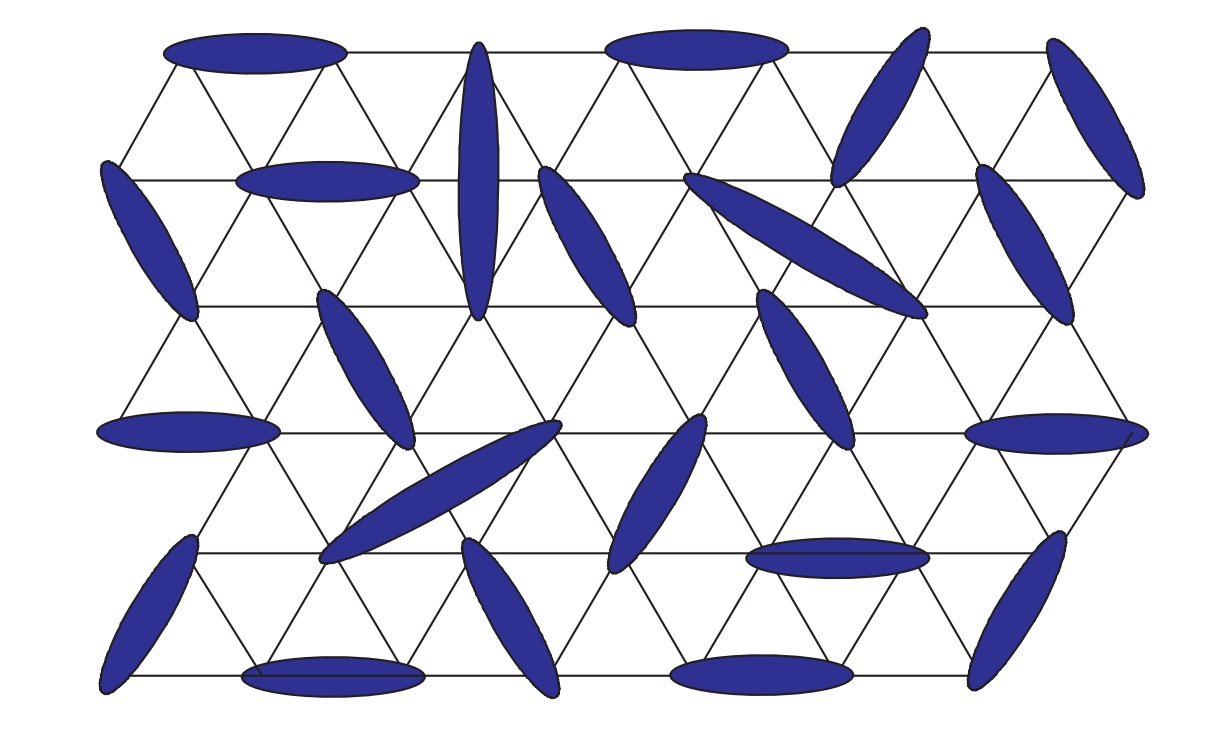
\includegraphics[width = 0.6\textwidth]{figures/RVB.jpg}
        \end{minipage}
        \begin{minipage}[l]{0.15\textwidth}
            \footnotesize{No magnetic order.}
            \vspace{.5cm}\\
            \tiny{Y. Zhou et al, Rev. Mod. Phys. (2017)}\hfill
        \end{minipage}
    \end{figure}
    \normalsize
     QSL can be characterized by topological order and long range entanglement. Signatures of QSL are mainly in the excitations with \emph{fractional quantum numbers} and anionic statistics. 
\end{frame}
\endgroup


\begin{frame}{Kitaev QSL}
    % \begin{columns}[t]
        % \column{0.7\textwidth} % Left column and width
            % \centering
        \begin{minipage}[c]{.6\textwidth}
            \begin{figure}
                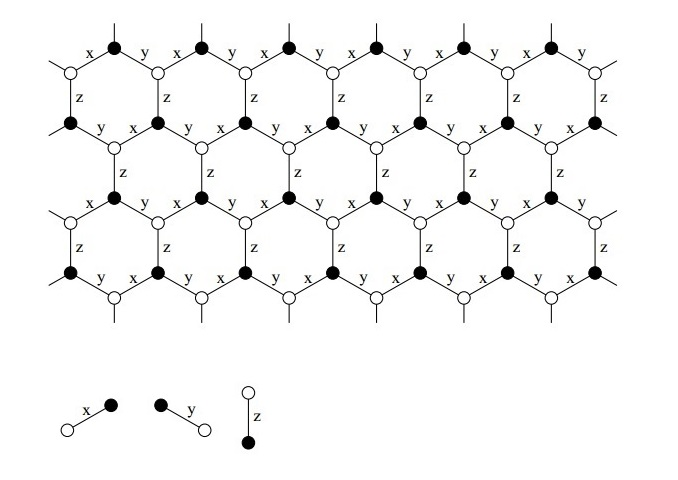
\includegraphics[width = 1\textwidth]{figures/1.jpg}
            \caption{\scriptsize A.Kitaev, Ann.Phys (2006)}
            \end{figure}
        \end{minipage}
        % \column{0.3\textwidth}
        \begin{minipage}[c]{.3\textwidth}
            \small
            % \vspace{1cm}
            1. Exactly solvable model with QSL ground state.\\
            % \\
            2. Experimental relevance: $\ch{(Na, Li)_2IrO_3}$, $\alpha\ch{-RuCl_3}$, $\ch{H_3LiIr_2O_6}$.
        \end{minipage}
    
    % \end{columns}
    
    \begin{flalign*}
        H = -J_x\sum_{x-links}\sigma_j^x\sigma_k^x  -J_y\sum_{y-links}\sigma_j^y\sigma_k^y  -J_z\sum_{z-links}\sigma_j^z\sigma_k^z
    \end{flalign*}
\end{frame}


\begin{frame}{Exact solution and Majorana fermions}
    \begin{figure}
    \centering
        \begin{minipage}[l]{.6\textwidth}
            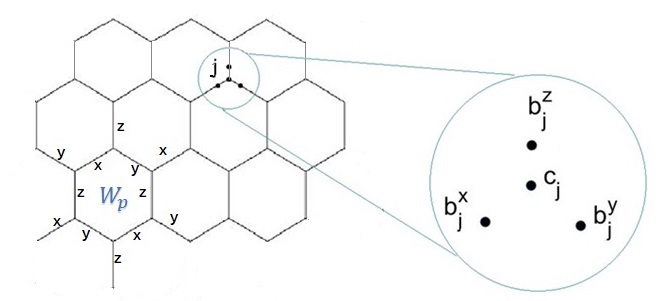
\includegraphics[width = 1\textwidth]{figures/lattice1.jpg}
        \end{minipage}
    \end{figure}


    \begin{columns}[t] % The "c" option specifies centered vertical alignment while the "t" option is used for top vertical alignment
    
    \column{0.5\textwidth} % Left column and width
    Large number of conserved quantities: local plaquette operator
    \begin{flalign*}
        W_p &= \sigma_1^x \sigma_2^y \sigma_3^z \sigma_4^x \sigma_5^y \sigma_6^z  & &\\
        [W_p, H] &= 0, \ [W_p, W_{p'}] = 0, \\ 
        W_p & \equiv \phi_p \pm 1, \\
        \ket{\psi} &= \ket{\{\phi_p\}} 
    \end{flalign*}
    
    \column{.5\textwidth} % Right column and width
    Majorana representation of spin-1/2.
    \begin{flalign*}
        \sigma_j^\alpha &= ib_j^\alpha c_j, \ \alpha = x, y, z 
    \end{flalign*}
    Quadratic Hamiltonian in each flux sector $\ket{\{\phi_p\}}$ :
    \begin{flalign*}
        H_u&= \frac{i}{2}\sum_{\left<i,j\right>}J_{\alpha_{ij}}\hat{u}_{ij}c_ic_j,\ \hat{u}_{ij} = ib_i^{\alpha_{ij}}b_j^{\alpha{ij}} &&
    \end{flalign*}
    
    \end{columns}

\end{frame}



\begin{frame}{Fractionalization of Kitaev spin liquid}

    \begin{columns}[t] 
        % The "c" option specifies centered vertical alignment while the "t" option is used for top vertical alignment
        
        \column{0.5\textwidth} % Left column and width
        Diagonalized $H_u$ in flux sector $\ket{\{\phi_p\}}$:
        \begin{flalign*}
            H_u &= \sum_i\epsilon_i(n_i-\frac{1}{2})
        \end{flalign*}
        The solution and the fractionalized excitations:
        \begin{flalign*}
            \ket{\psi} &= \ket{\{\phi_p\}, \{n_i\}}
        \end{flalign*}
        $\phi_p = -1$: $Z_2$ flux flux configuration.\\
        % $\phi_p = -1$: $Z_2$ flux\\
        $n_i$: fermionic numbers.\\
        The ground state is the flux-free state.
        $\ket{\leftc \phi_p = +1 \rightc}$
        
        
        \column{.5\textwidth} % Right column and width
        % Realization of a flux configuration with $u_{jk}$ operators:
        % \begin{align*}
        %     W_p & = \prod_{(j,k)\in edge(p)} \hat{u}_{jk}
        % \end{align*}
        $\leftc\phi_p\rightc$:
        \begin{figure}
            \centering
            \begin{minipage}[l]{.7\textwidth}
                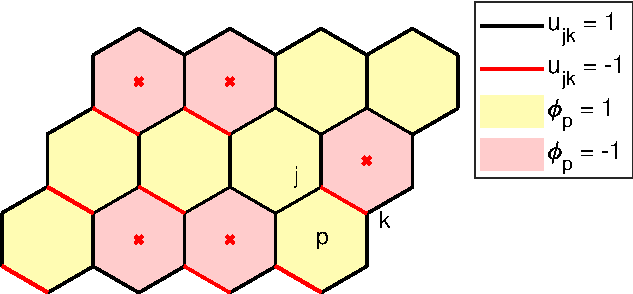
\includegraphics[width = 1\textwidth]{figures/lattice2.pdf}
            \end{minipage}
        \end{figure}
        \vspace{.5cm}
        $\leftc n_i \rightc$:
        \begin{figure}
            \centering
            \begin{minipage}[l]{.6\textwidth}
                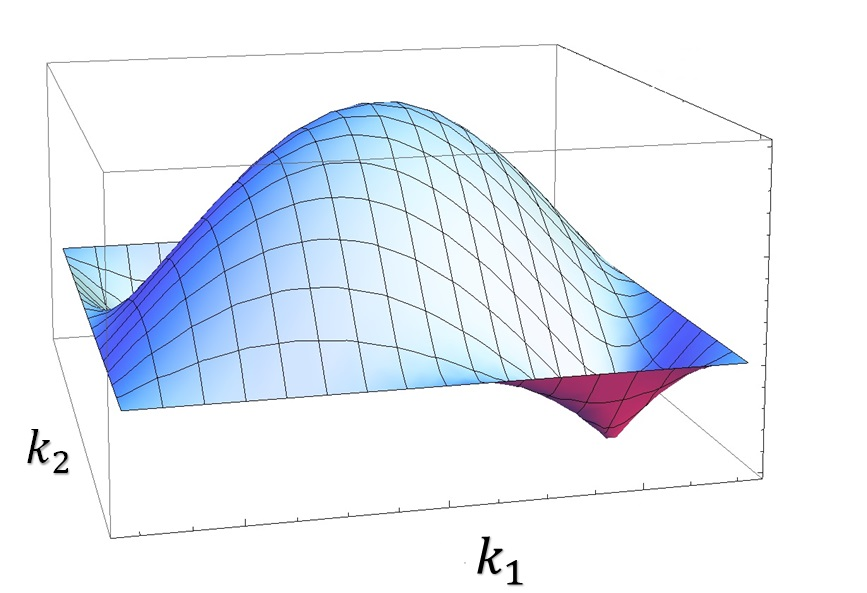
\includegraphics[width = 1\textwidth]{figures/torus_band.jpg}
            \end{minipage}
        \end{figure}
    \end{columns}
\end{frame}


\begin{frame}{Fractionalization at finite temperature}

    \begin{figure}
    \centering
        \begin{minipage}[t]{.85\textwidth}
            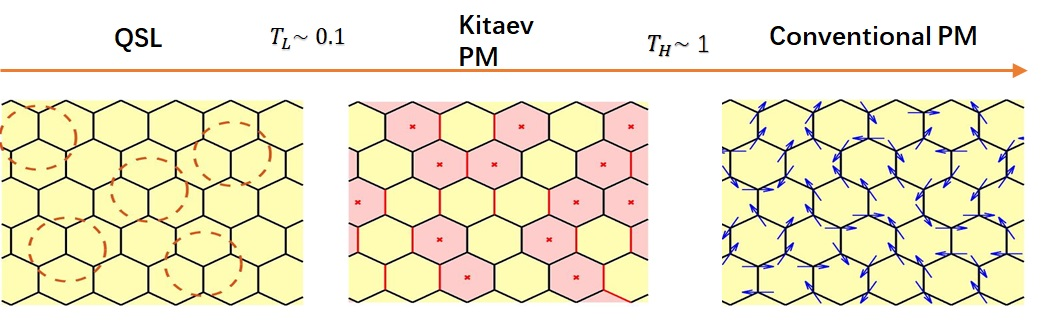
\includegraphics[width = 1\textwidth]{figures/TLTH.jpg}
        \end{minipage}
    \end{figure}
    
    Fractionalized spin excitations: $\ket{\leftc\phi_p\rightc, \leftc n_i\rightc}$, $Z_2$ flux and MF.
    
    \begin{columns}[c]
    \column{0.8\textwidth}
    \begin{figure}[t]
        \centering
        % \begin{minipage}[t]{\textwidth}
        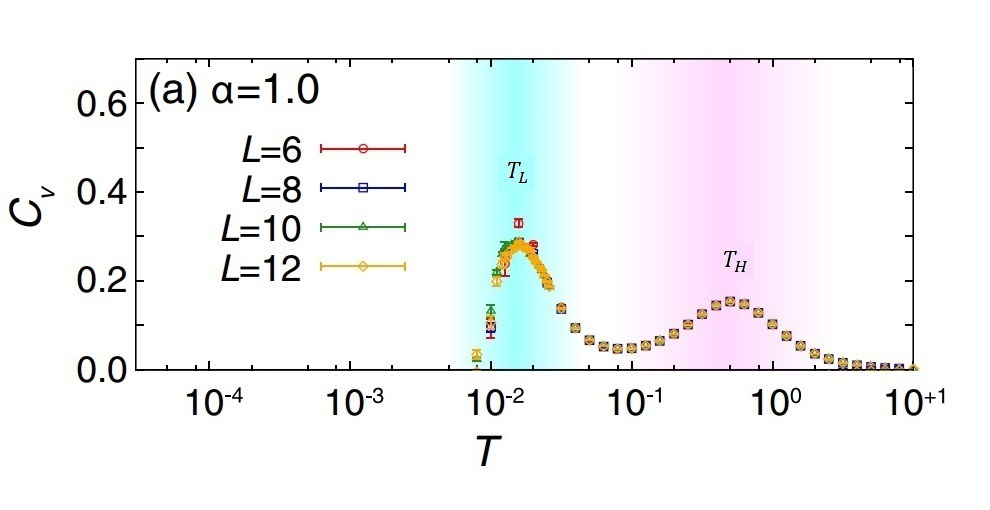
\includegraphics[width = .75\textwidth]{figures/Cv2.jpg}
        % \end{minipage}
    \end{figure}
    
    \column{0.2\textwidth}
        % \vspace{3cm}
        \scriptsize J.Nasu, et al PRB (2015)
    \end{columns}
    
\end{frame}



\begin{frame}{Specific heat from MC calculation.}
    % The thermodynamic distribution of the excitations:
    % \begin{flalign*}
    %     p(\{\phi_p\}, \{n_i\}) &\sim e^{-\beta \sum_i \epsilon_i(n_i - \oh) } = e^{-\beta [-\oh \sum_i \epsilon_i + \sum_i n_i \epsilon_i]}
    %     % Z = \sum_{\{\phi_p\}, \{n_i\}} e^{-\beta E()}
    %     % \lefta E \righta &= Tr(H e^{-\beta H}), \quad C = \frac{\partial \lefta E \righta}{\partial T}
    % \end{flalign*}
    % Flux energy: $E_{\tx{flux}} \equiv = -\oh \sum_i \epsilon_i$
    
    \begin{figure}
        \centering
        \begin{minipage}[l]{.8\textwidth}
            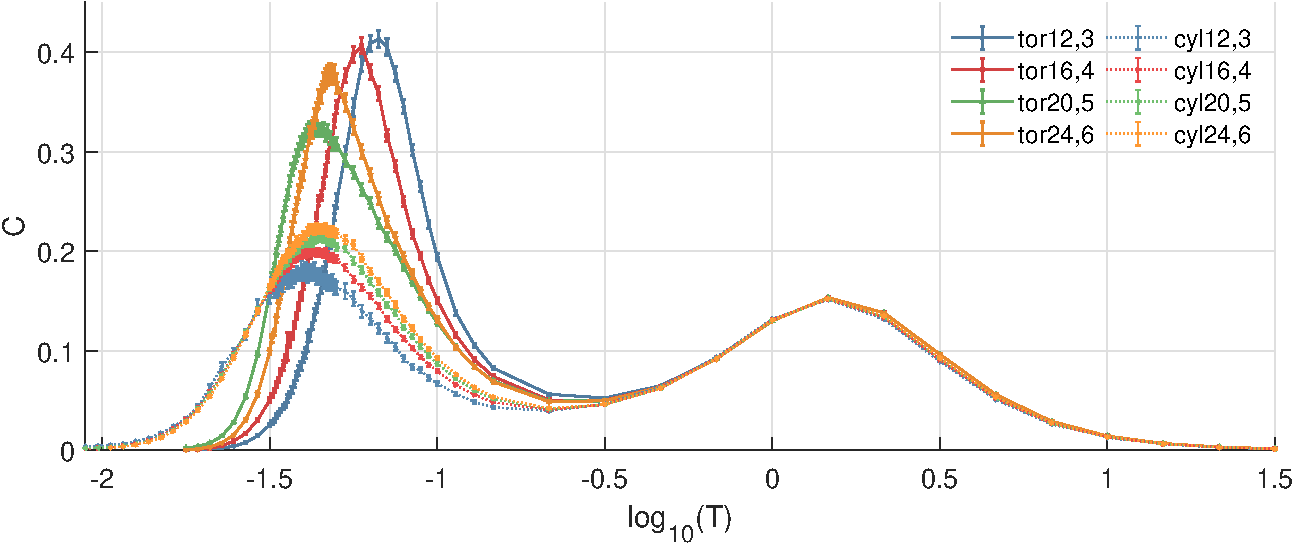
\includegraphics[width = 1\textwidth]{figures/Cv_all.pdf}
        \end{minipage}
    \end{figure}
    % What physics effect does the $T_L$ peak display? How is it related to the flux energetics.
    Objective: flux energetics dependence on lattice geometries, ie.\ torus and cylinder, and lattice sizes. 
\end{frame}


\begin{frame}{A brief introduction of MC algorithm}
    The probability distribution of a flux config.:
    $$p(\leftc \phi_p\rightc) \sim e^{-\beta F(\leftc\phi_p\rightc)}$$
    
    A sequence of flux config.\ samples (Markov Chain):
    \begin{figure}
        \centering
        \begin{minipage}[t]{.6\textwidth}
            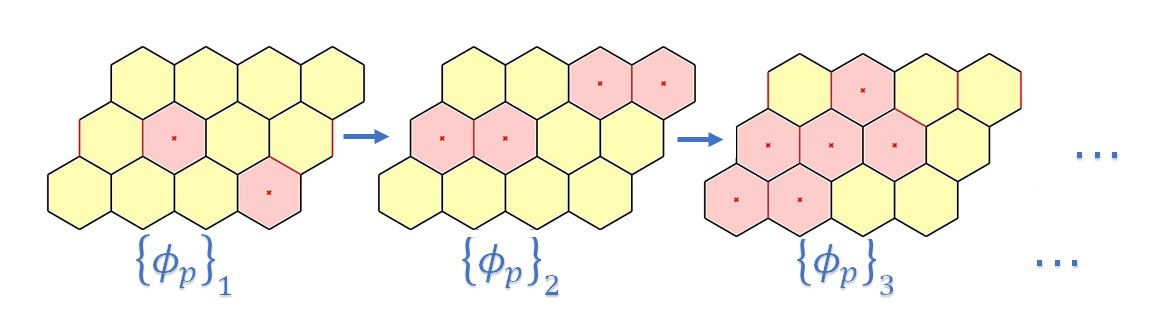
\includegraphics[width = \textwidth]{figures/config1.jpg}
        \end{minipage}
    \end{figure} 
    \begin{align*}
        C &= \onefrac{T^{2}}\left(\lefta E_{F}^{2}\righta-\lefta E_{F}\righta^{2} - \lefta\frac{\partial E_{F}}{\partial \beta}\righta\right) 
    \end{align*}
    $\lefta\ldots\righta$ is taken over all the samples of flux config.\ $\leftc\phi_p\rightc_i$. $E_F = E_F(\leftc\phi_p\rightc)$.
    
    % Metropolis-Hasting update: $T(\leftc\phi_p\rightc_1 \to \leftc\phi_p\rightc_2) = \min\leftc 1, \frac{p(\leftc\phi_p\rightc_2)}{p(\leftc\phi_p\rightc_1)}\rightc $
\end{frame}


%%%%%%%%%%%%%%%%%%%%%%%%%%%%%%%%%%%%%
\section{Phenomenological study of the flux energetics}
\begin{frame}
\centerline{2. Phenomenological study of the flux energetics}
\end{frame}




\begin{frame}{Distributions of flux energies on torus}
    % The thermodynamic distribution of the excitations:
    % \begin{flalign*}
    %     % p(\{\phi_p\}) &\sim e^{-\beta \sum_i \epsilon_i(n_i - \oh) } = e^{-\beta [-\oh \sum_i \epsilon_i + \sum_i n_i \epsilon_i]}
    %     p(\{\phi_p\}) &\sim e^{-\beta (-\oh \sum_i \epsilon_i) + \sum_i \ln(1+e^{-\beta \epsilon_i})}
    %     % Z = \sum_{\{\phi_p\}, \{n_i\}} e^{-\beta E()}
    %     % \lefta E \righta &= Tr(H e^{-\beta H}), \quad C = \frac{\partial \lefta E \righta}{\partial T}
    % \end{flalign*}
    Flux energy: $E_{\tx{flux}}(\leftc\phi_p\rightc) \equiv = -\oh \sum_i \epsilon_i$
    
    \begin{figure}
        \centering
        \begin{minipage}[c]{.6\textwidth}
            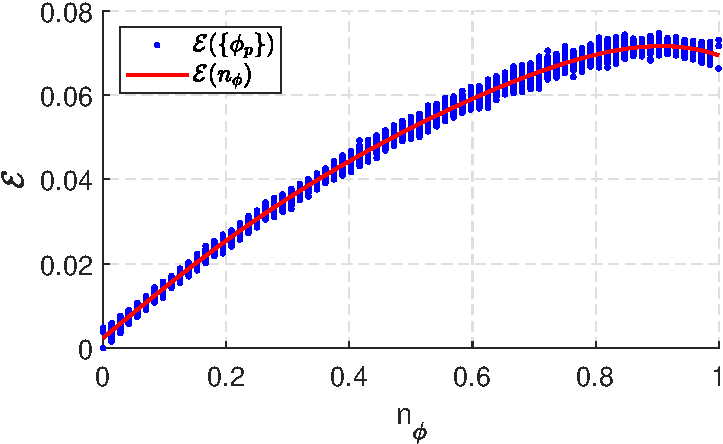
\includegraphics[width = 1\textwidth]{figures/24_6_tor.pdf}
        \end{minipage}
        % \begin{minipage}[c]{.45\textwidth}
        %     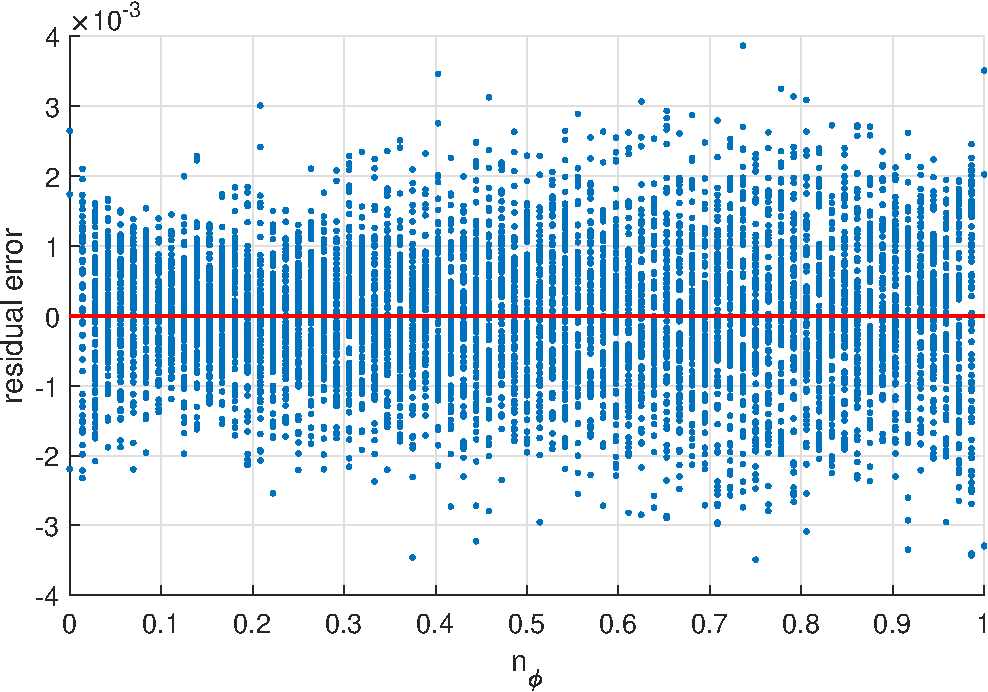
\includegraphics[width = 1\textwidth]{figures/cir_24_wid_6_deg_5_percent_1_res.pdf}
        % \end{minipage}
        \caption{Flux energies obtained by sampling the flux configurations with equal probability. 100 data points for each flux density.}
    \end{figure}
    Interacting flux model on torus (IFMT).

\end{frame}

\begin{frame}
\begin{figure}
    \centering
    \begin{minipage}[c]{.45\textwidth}
        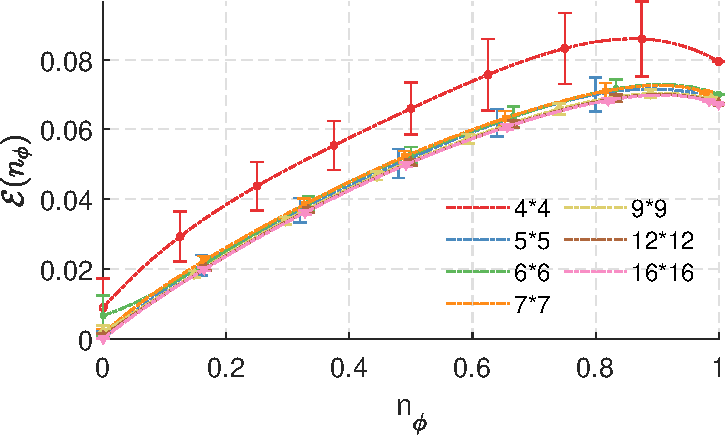
\includegraphics[width = 1\textwidth]{figures/band_extrapolation_1.pdf}
    \end{minipage}
        \begin{minipage}[c]{.45\textwidth}
        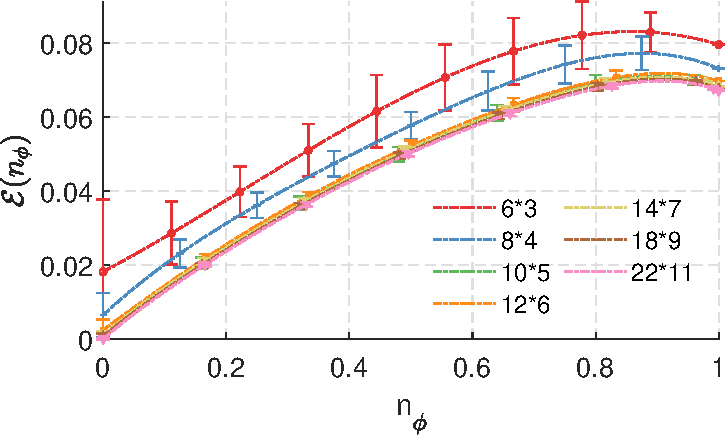
\includegraphics[width = 1\textwidth]{figures/band_extrapolation_2.pdf}
    \end{minipage}
        \begin{minipage}[c]{.45\textwidth}
        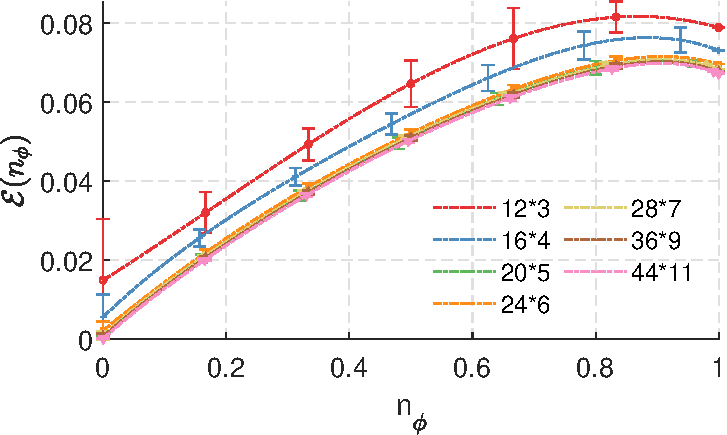
\includegraphics[width = 1\textwidth]{figures/band_extrapolation_4.pdf}
    \end{minipage}
    \begin{minipage}[c]{.45\textwidth}
        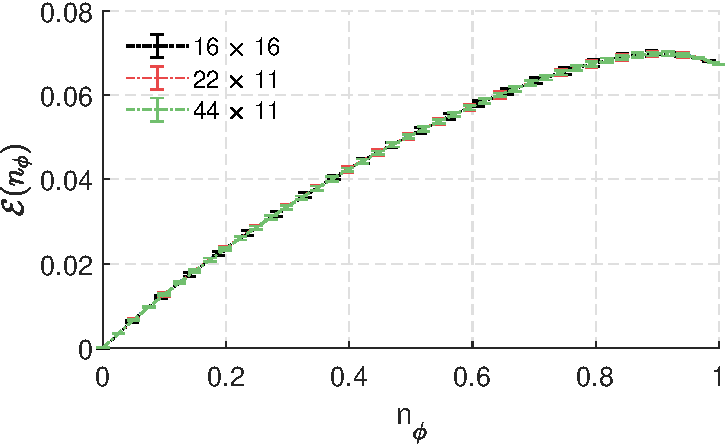
\includegraphics[width = 1\textwidth]{figures/limit_band.pdf}
    \end{minipage}
\end{figure}
\hfill Universal lattice-size-independent flux energy model.

    % Approximate flux energy models:\\
    % Interacting flux model (IFMT):  $\E(n_\phi) = \Delta \nphi$\\
    % Non-interacting flux model (NIFMT): $\E(\nphi) = -0.14 \nphi^5 + 0.27 \nphi^4 - 0.18 \nphi^3 - 0.0037 \nphi^2 + 0.12 \nphi + 0.0024$
    % The best fit pseudopotential energy:
    % \begin{align*}
    %     \E(\nphi) &= -0.32\nphi^6 + 0.85\nphi^5 - 0.9\nphi^4 + 0.48\nphi^3 - 0.18\nphi^2 + 0.14\nphi + 0.000011.
    % \end{align*}
\end{frame}



\begin{frame}{Phenomenological flux energy models}
    \begin{figure}
        \centering
        \begin{minipage}[c]{.7\textwidth}
            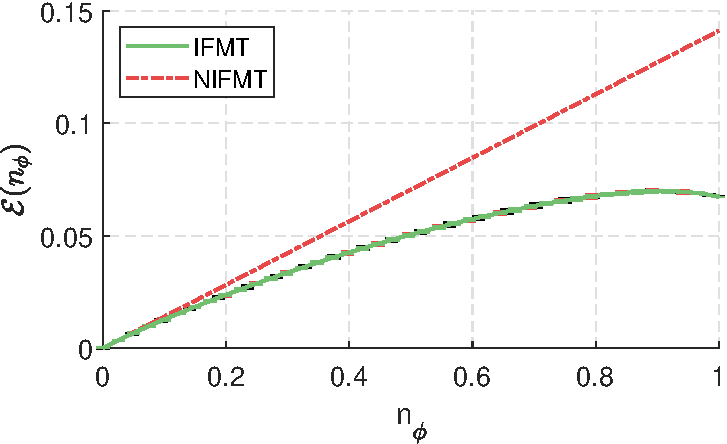
\includegraphics[width = 1\textwidth]{figures/limit_poly_linear.pdf}
        \end{minipage}
    \end{figure}

    Phenomenological flux energy models:\\
    Interacting flux model (IFMT): $\E(\nphi) = -0.32\nphi^6 + 0.85\nphi^5 - 0.9\nphi^4 + 0.48\nphi^3 - 0.18\nphi^2 + 0.14\nphi + 0.000011$
    Non-interacting flux model (NIFMT):  $\E(n_\phi) = \Delta_\phi \nphi$, $\Delta_\phi = 0.14$.\\
\end{frame}



\begin{frame}{The specific heat of flux models}
The free energy:
\begin{align*}
    F &= E_{\tx{flux}} - TS = N_p\left(\E(\nphi) - \frac{T}{N_p}\ln{{N_p \choose N_\phi}}\right)
    % S & = N_p\left[-\nphi\ln{\nphi} - (1 - \nphi) \ln{(1-\nphi)}\right], \quad N_p \gg 1
\end{align*}
The saddle-point solution $\ud F/\ud n_\phi = 0 \Rightarrow \nphi = \nphi(T)$:
\begin{align*}
    % 0 &= \E'(\nphi) - T\ln{\frac{1-\nphi}{\nphi}}\\
    \C &= \frac{\ud \E(\nphi)}{\ud T} = \frac{\E'(\nphi)^2}{T^2}\onefrac{\onefrac{\nphi(1-\nphi)} + \frac{\E''(\nphi)}{T}}
\end{align*} 
Non-interacting model (NIFMT) : $\E''(\nphi) = 0$.\\
Interacting model (IFMT): $\E''(\nphi) < 0$ (attractive interaction) \\


% Flux onset temperature:
% \begin{align*}
%     T_\phi &= \frac{\E'(0)}{\n N_p} = \frac{\Delta_\phi}{\ln N_p}
% \end{align*}
\end{frame}


\begin{frame}{Comparison with the actual specific heat}
    \begin{figure}
        \centering
        \begin{minipage}[c]{.8\textwidth}
            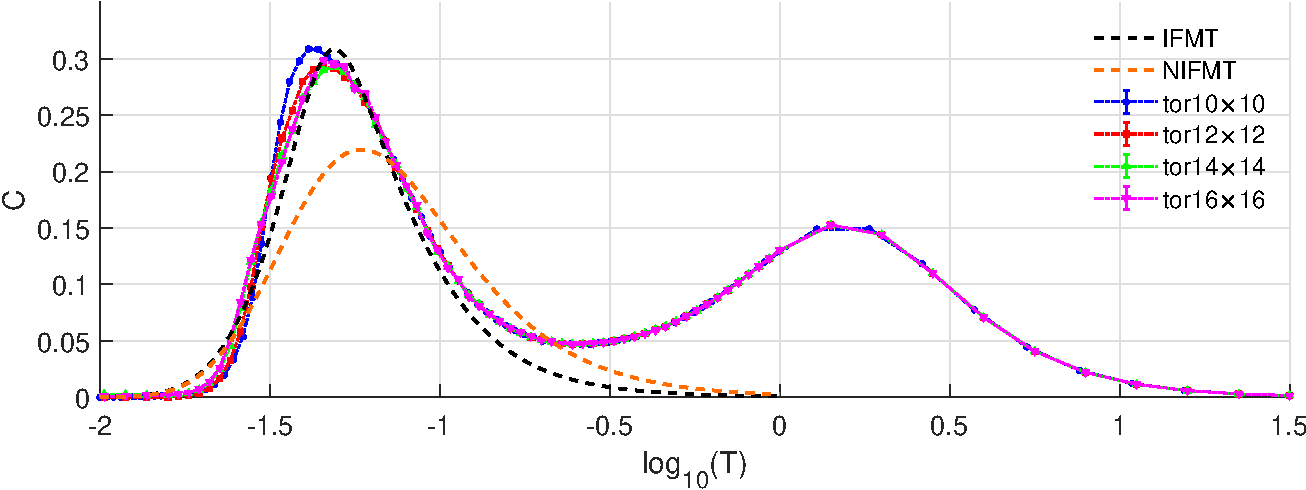
\includegraphics[width = 1\textwidth]{figures/thermo_limit_C.pdf}
        \end{minipage}
    \end{figure}
    Flux attractive interaction increases thermal fluctuations. \\
    The interacting flux model (IFMT) is able to capture most of the thermal fluctuations. 
\end{frame}


\begin{frame}{Flux energy models on cylinder}
    \small
    Effective attraction from the edge.
    \begin{figure}
        \centering
        \begin{minipage}[c]{.4\textwidth}
            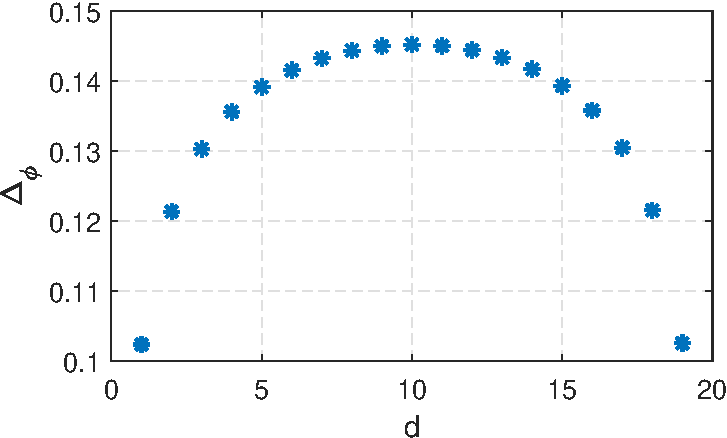
\includegraphics[width = 1\textwidth]{figures/flux_potential_dy_40_20.pdf}
        \end{minipage}
        \hspace{0.3cm}
        \begin{minipage}[c]{.4\textwidth}
            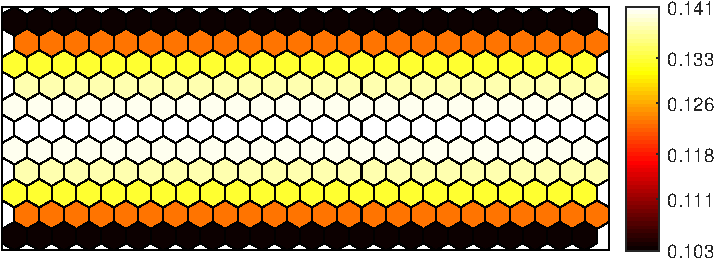
\includegraphics[width = 1\textwidth]{figures/one_flux.pdf}
        \end{minipage}

        \begin{minipage}[t]{.4\textwidth}
            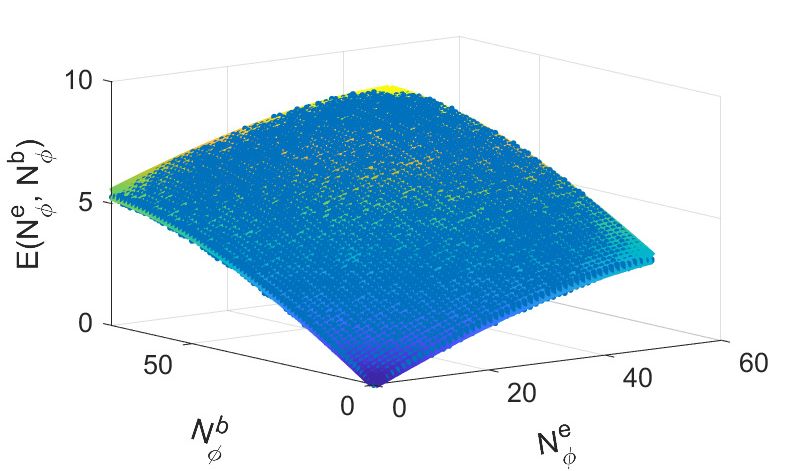
\includegraphics[width = 1\textwidth]{figures/cyl_cir_24_wid_6.pdf}
        \end{minipage}
        \begin{minipage}[t]{.15\textwidth}
            % \vspace{2cm}
            \footnotesize $24\times 6$ lattice
        \end{minipage}
    \end{figure}
    
    \small
    Interacting flux model (IFMC): $E_\tx{flux} = E_\tx{flux}(N^e_\phi, N^b_\phi)$ \\
    Non-interacting flux model (NIFMC): $E_\tx{flux}= \Delta_\phi^e N_\phi^e + \Delta_\phi^b N_\phi^b$ \\
    % $\Delta_\phi^e = 0.10$, $\Delta_\phi^b = 0.14$
\end{frame}



\begin{frame}{The effect of open boundaries on the specific heat}
    \begin{figure}
        \centering
        \begin{minipage}[c]{.75\textwidth}
            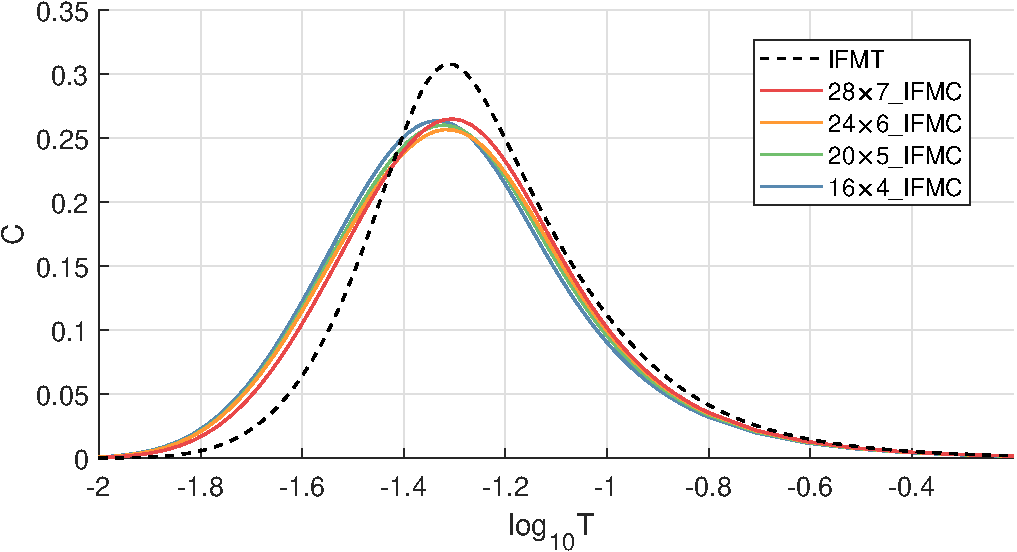
\includegraphics[width = 1\textwidth]{figures/C_cyltor.pdf}
        \end{minipage}
    \end{figure}
    \begin{columns}[t]
        \column{.5\textwidth}
         Edge fluxes have lower energy. The entropy release is more gradually on cylinder. $C = \ud S/ \ud \log T$.
        
        \column{.5\textwidth}
        \begin{figure}[t]
            % \begin{minipage}[t]{.7\textwidth}
            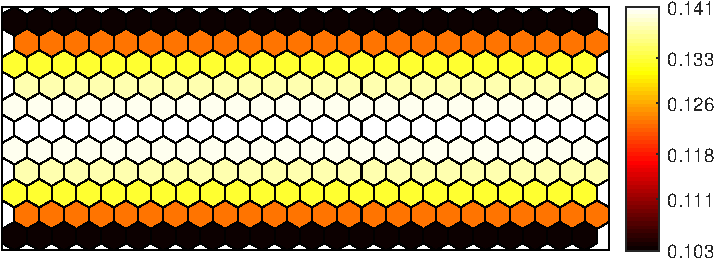
\includegraphics[width = .7\textwidth]{figures/one_flux.pdf}
            % \end{minipage}
        \end{figure} 
    \end{columns}
\end{frame}


\begin{frame}{Comparison of IFMC with MC}
    \begin{figure}
        \centering
        \begin{minipage}[c]{.7\textwidth}
            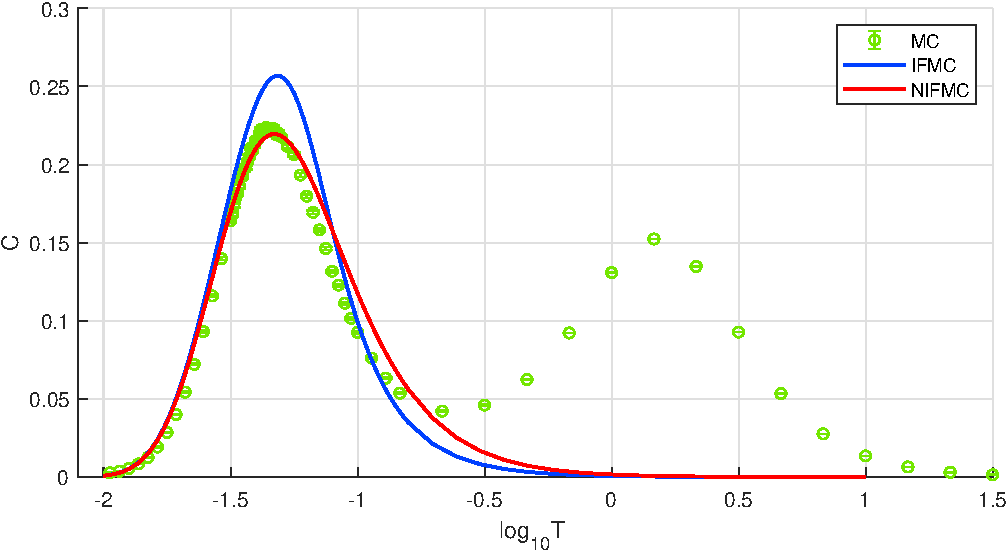
\includegraphics[width = 1\textwidth]{figures/C_cir_24_wid_6_cyl.pdf}
        \end{minipage}
    \end{figure}
    \begin{columns}[t]
        \column{0.3\textwidth} % Left column and width
            % \vspace{1cm}
            \begin{center}
                The edge fluxes decrease the specific heat.
            \end{center}
        \column{0.7\textwidth}
            \begin{figure}
                \begin{minipage}[c]{.5\textwidth}
                    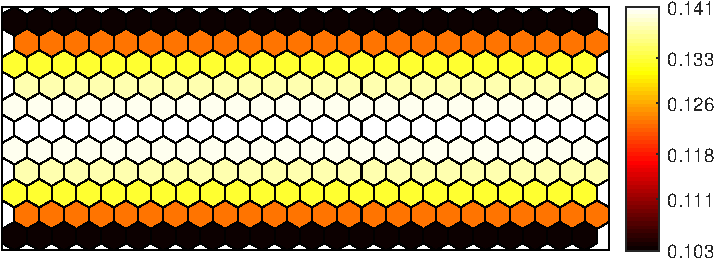
\includegraphics[width = 1\textwidth]{figures/one_flux.pdf}
                \end{minipage}
            \end{figure}   
    \end{columns}
\end{frame}




%%%%%%%%%%%%%%%%%%%%%%%%%%%%%%%%%%%%

\section{Two-flux interaction and magnetic field}

\begin{frame}
    3. Two-flux interaction and the effect of magnetic field.
    \begin{figure}
        \centering
        \begin{minipage}[c]{.5\textwidth}
            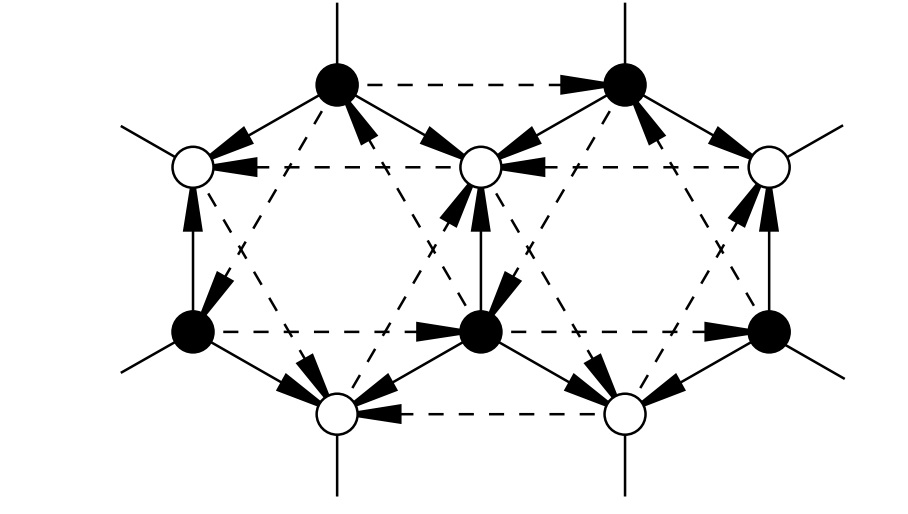
\includegraphics[width = .75\textwidth]{figures/three-spin.jpg}
        \end{minipage}
    \end{figure}
    \begingroup
    \small
        \begin{align*}
            H & = -\sum_{\langle i, j\rangle}J^{\alpha_{ij}} \sigma_i^{\alpha_{ij}} \sigma_j^{\alpha_{ij}} - \kappa \sum_{<i,j,k>} \sigma^x_i \sigma^y_j \sigma^z_k 
            % & = \frac{i}{4} \sum_{\langle i, j\rangle} h_{ij} c_i c_j, \quad h_{ij} = 2J^{\alpha_{ij}} \hat{u}_{ij}+ 2\kappa\hat{u}_{ik}\hat{u}_{jk}
        \end{align*}
    \endgroup
\end{frame}

\begin{frame}{Two-flux interaction}
    \begin{figure}
        \begin{minipage}[c]{.45\textwidth}
            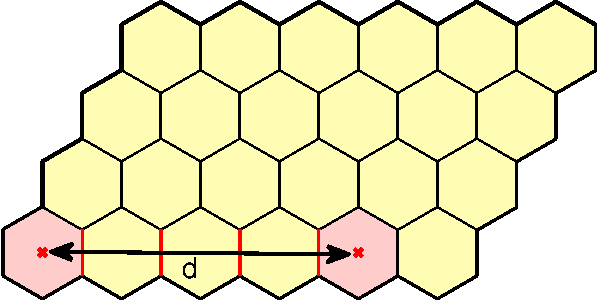
\includegraphics[width = 1\textwidth]{figures/lattice_tor_2flux.pdf}
            \vspace{.8cm}
        \end{minipage}
        \begin{minipage}[c]{.45\textwidth}
            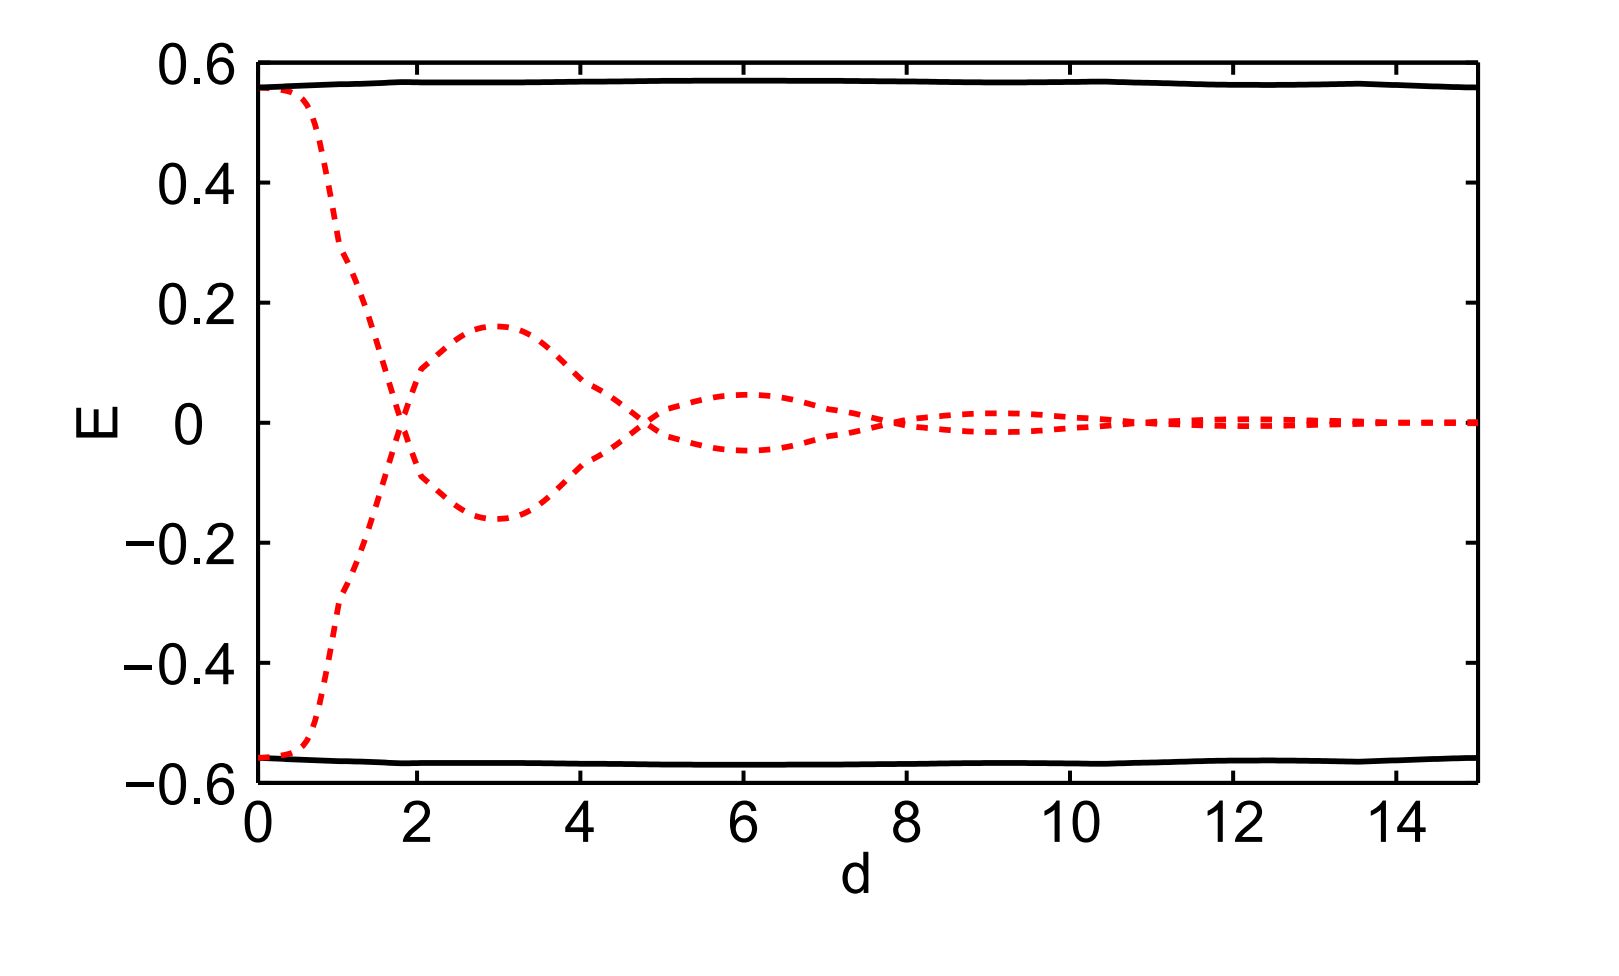
\includegraphics[width = 1\textwidth]{figures/interaction.png}
        \end{minipage}
    \end{figure}
    \begin{align*}
        E^d_{int} &= \Delta_f \cos\left(\frac{2\pi d}{\lambda}\right) e^{-\frac{d}{\xi}}, \ \xi \sim \kappa ^{-1}
    \end{align*}
    Exponential decaying amplitude. Short-range interaction.\\
    \footnotesize{V. Lahtinen, el at, New Jour. Phys. (2011)}
\end{frame}




\begin{frame}
    \footnotesize
    \begin{figure}
        \subfigure[$\kappa = 0$]{
        \begin{minipage}[c]{.4\textwidth}
            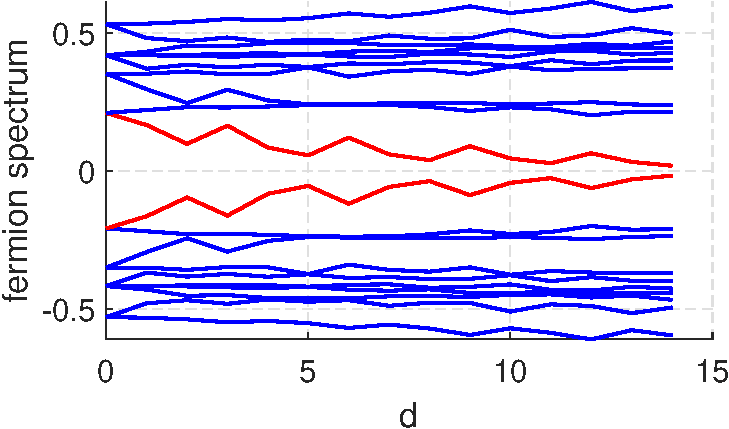
\includegraphics[width = 1\textwidth]{figures/Fermion_spectrum_vs_dx_0.pdf}
        \end{minipage}
        }
        \subfigure[$\kappa=0.5$]{
        \begin{minipage}[c]{.4\textwidth}
            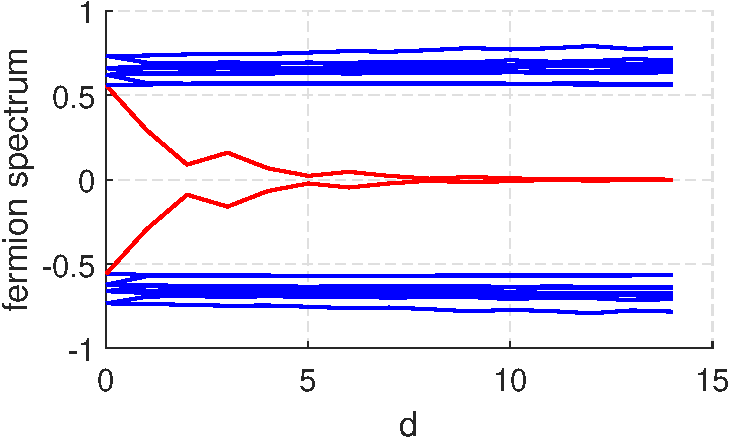
\includegraphics[width = 1\textwidth]{figures/Fermion_spectrum_vs_dx_5.pdf}
        \end{minipage}
        }
    
        \subfigure[$\kappa = 0$]{
        \begin{minipage}[c]{.4\textwidth}
            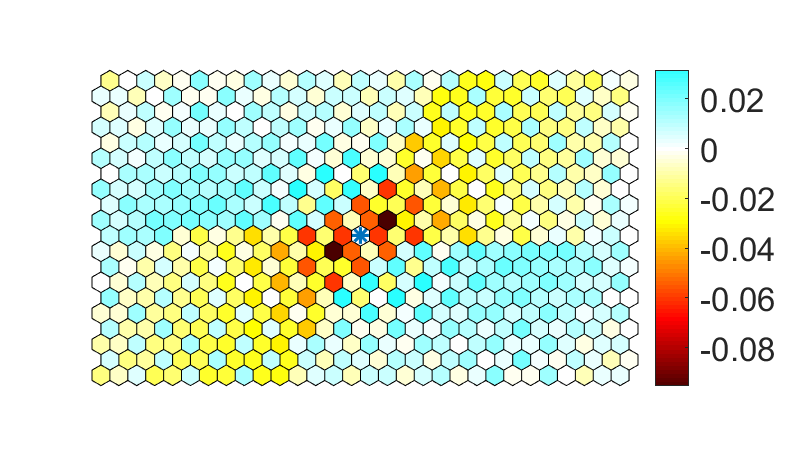
\includegraphics[width = 1\textwidth]{figures/cir_30_wid_20_topsec_-1_kap_0.pdf}
        \end{minipage}
        }
        \subfigure[$\kappa = 0.5$]{
        \begin{minipage}[c]{.4\textwidth}
            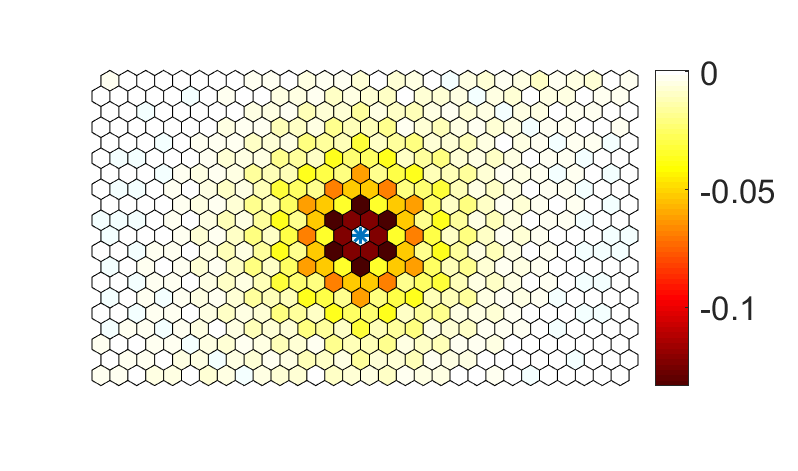
\includegraphics[width = 1\textwidth]{figures/cir_30_wid_20_topsec_-1_kap_5.pdf}
        \end{minipage}
        }
    \end{figure}
    % Flux interaction: $E^d_{int} = E^d_{2\phi} - E^{\infty}_{2\phi}$, $E^d_{2\phi} = - \oh \sum \epsilon_i$.
    % \footnotesize
    
    \begin{align*}
        E^d_{int} &= \Delta_f \cos\left(\frac{2\pi d}{\lambda}\right) e^{-\frac{d}{\xi}}, \ \xi \sim \kappa ^{-1}
    \end{align*}
    


\end{frame}


\begin{frame}{The effect of magnetic field on flux energy}
    \begin{figure}
        \begin{minipage}[l]{.45\textwidth}
            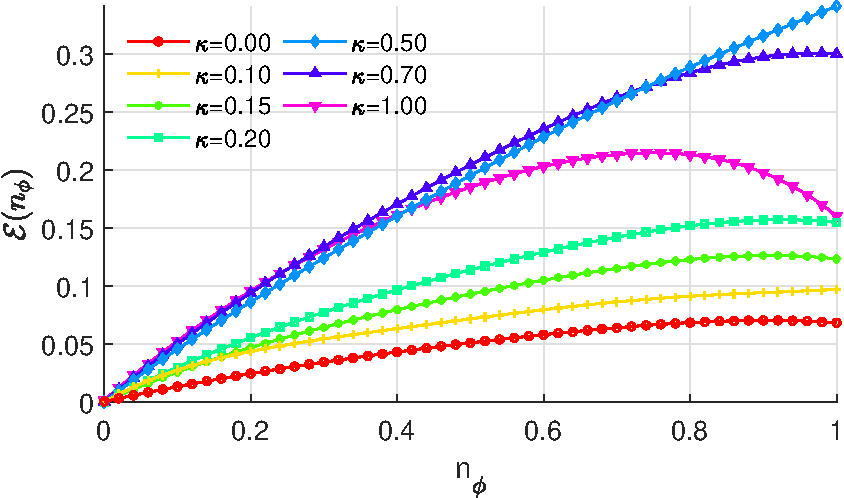
\includegraphics[width = 1\textwidth]{figures/band_extrapolation.pdf}
        \end{minipage}
        \begin{minipage}[t]{.35\textwidth}
            \footnotesize
            \hspace{0.5cm}$\xi\sim\kappa^{-1}$ invalid for $\kappa>0.5$
        \end{minipage}
        
        \begin{minipage}[c]{.7\textwidth}
            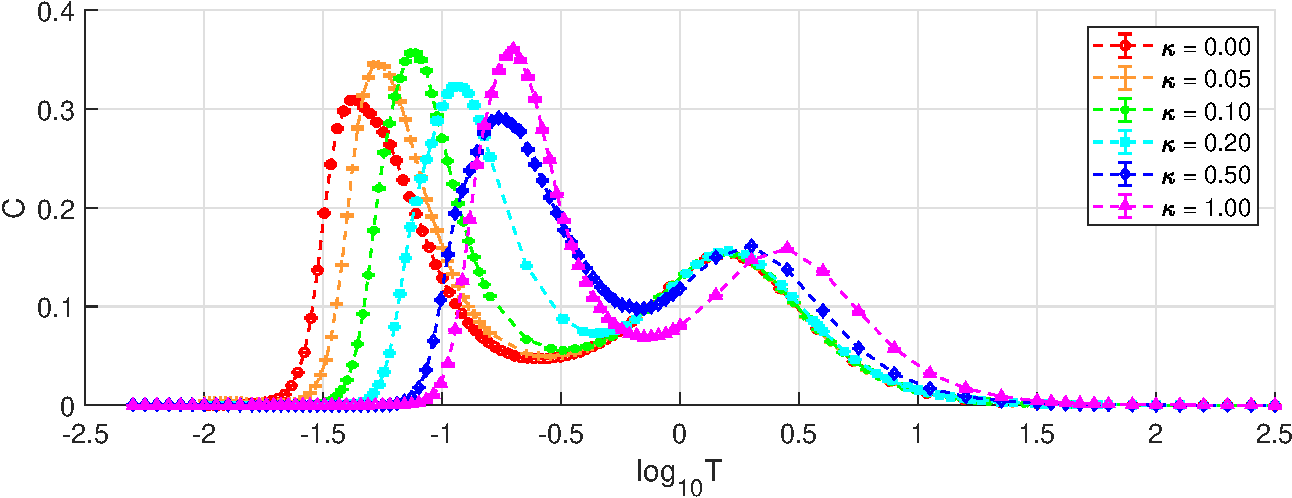
\includegraphics[width = 1\textwidth]{figures/Cv_10_10.pdf}
        \end{minipage}
    \end{figure}
    \centering \small $\Delta_\phi = \E'(0)$
\end{frame}


\begin{frame}
\large
\centerline{Thank you!}
\end{frame}